\documentclass[11pt]{article}
\usepackage[margin=1in]{geometry}
\usepackage{amsmath,amssymb,booktabs,array,longtable}
\usepackage{graphicx}
\usepackage{hyperref}
\usepackage{enumitem}
\usepackage{titlesec}

\begin{document}

\begin{center}
\Large\textbf{Shiv Nadar University Chennai}\\[2mm]
\end{center}

\renewcommand{\arraystretch}{1.4}

\begin{tabular}{|p{3.5cm}|p{8cm}|p{2cm}|}
\hline
Degree \& Branch & B.Tech Artificial Intelligence \& Data Science & Semester V\\ \hline
Subject Code \& Name & CS3807 -- Deep Learning Laboratory & AY: 2026--27\\ \hline
\end{tabular}

\vspace{3mm}

\begin{center}
\Large\textbf{Experiment 1}\\
\large\textbf{Implementation of a Single Layer Perceptron for Binary Classification}
\end{center}

%----------------------------------------------------------

\section*{1. Objective}

The objective of this experiment is to understand the concept of an artificial neuron and implement a Single Layer Perceptron from scratch for binary classification. Students will learn the perceptron learning algorithm, understand the importance of activation functions, visualize the learning process, and evaluate the classifier using a real-world dataset.

%----------------------------------------------------------

\section*{2. Background Theory}

An Artificial Neuron is the fundamental building block of a neural network. It receives one or more input features, multiplies them by corresponding weights, adds a bias term, and applies an activation function to determine the output.

The Single Layer Perceptron is the earliest supervised learning algorithm capable of solving linearly separable binary classification problems.

\subsection*{Mathematical Formulation}

Weighted Sum

\[
z=\mathbf{w}^{T}\mathbf{x}+b
\]

where

\begin{itemize}
\item $\mathbf{x}$ : Input vector
\item $\mathbf{w}$ : Weight vector
\item $b$ : Bias
\item $z$ : Linear combination
\end{itemize}

Prediction

\[
\hat y=f(z)
\]

Weight Update Rule

\[
\mathbf{w}_{new}
=
\mathbf{w}_{old}
+
\eta
(y-\hat y)
\mathbf{x}
\]

Bias Update

\[
b_{new}
=
b_{old}
+
\eta
(y-\hat y)
\]

where $\eta$ denotes the learning rate.

%----------------------------------------------------------

\section*{3. Activation Functions}

An activation function determines the output of a neuron based on the weighted sum of its inputs. It introduces non-linearity, enabling neural networks to learn complex patterns. Although the perceptron uses only the Step Activation Function, modern deep learning models employ differentiable activation functions for efficient optimization through backpropagation.

\subsection*{Step Activation Function}

\[
f(z)=
\begin{cases}
1,&z\ge0\\
0,&z<0
\end{cases}
\]

The Step Activation Function produces a binary output and is therefore suitable only for linearly separable binary classification problems.

\begin{center}
\begin{tabular}{|p{2.5cm}|p{3cm}|p{6cm}|}
\hline
\textbf{Activation} & \textbf{Output Range} & \textbf{Typical Applications}\\
\hline
Step & $\{0,1\}$ & Classical Perceptron\\
\hline
Sigmoid & $(0,1)$ & Binary Classification Output Layer\\
\hline
Tanh & $(-1,1)$ & Hidden Layers (Traditional Networks)\\
\hline
ReLU & $[0,\infty)$ & Hidden Layers in CNNs and MLPs\\
\hline
Leaky ReLU & $(-\infty,\infty)$ & Avoiding Dying ReLU\\
\hline
Softmax & $(0,1)$ & Multi-class Classification Output Layer\\
\hline
\end{tabular}
\end{center}

\textbf{Note:} This experiment uses only the Step Activation Function. The remaining activation functions will be studied in subsequent experiments involving Multilayer Perceptrons and Deep Neural Networks.

%----------------------------------------------------------

\section*{4. Dataset Description}

\textbf{Dataset:} Banknote Authentication Dataset

\textbf{Source:} UCI Machine Learning Repository

\textbf{Download Link:}

\url{https://archive.ics.uci.edu/dataset/267/banknote+authentication}

\begin{center}
\begin{tabular}{|l|l|}
\hline
Instances & 1372\\
\hline
Features & 4 Numerical Features\\
\hline
Classes & 2\\
\hline
Missing Values & None\\
\hline
Task & Binary Classification\\
\hline
\end{tabular}
\end{center}

\textbf{Feature Description}

\begin{itemize}
\item Variance
\item Skewness
\item Curtosis
\item Entropy
\end{itemize}

Target Class

\begin{itemize}
\item 0 -- Authentic Banknote
\item 1 -- Forged Banknote
\end{itemize}

%----------------------------------------------------------

\section*{5. Source Code}

The complete source code for this experiment is available at the following GitHub repository:

\url{https://github.com/your-username/your-repository}

%----------------------------------------------------------

\section*{6. Generated Plots with Interpretation}

\begin{center}
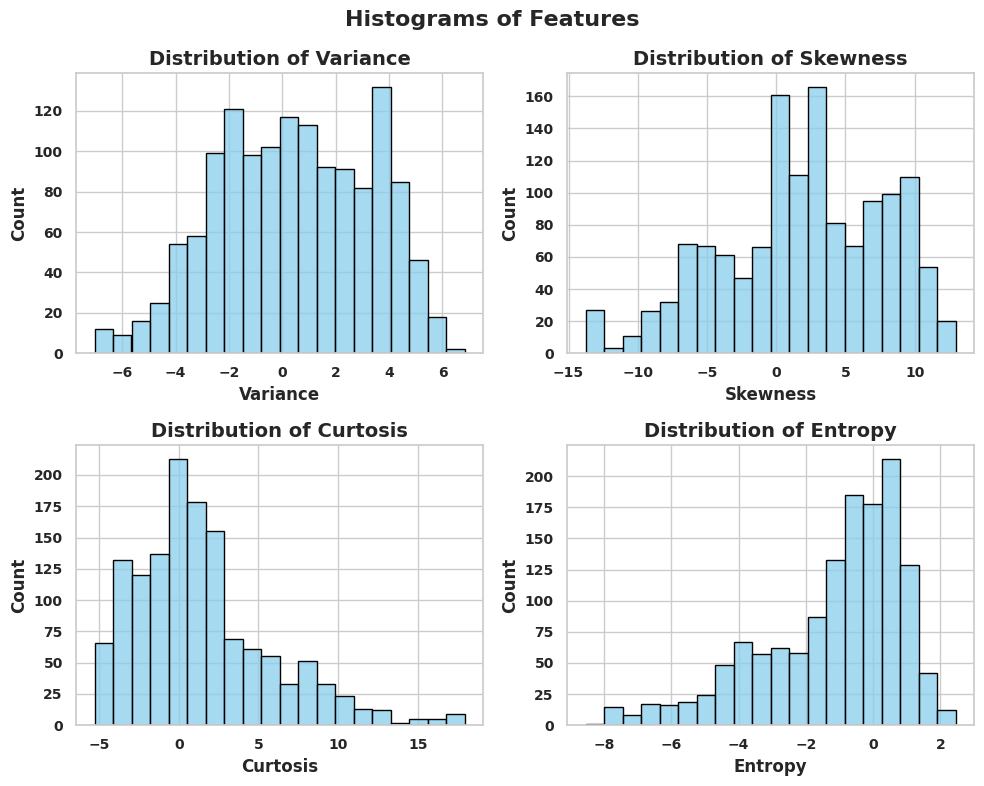
\includegraphics[width=0.75\textwidth]{Histograms.png}
\end{center}

The histograms reveal that Variance and Entropy are roughly symmetric but multi-modal, whereas Skewness and Curtosis are noticeably right-skewed with a long tail of large positive values. This spread in shape and scale across features confirms the need for normalization before training the perceptron.

\vspace{4mm}

\begin{center}
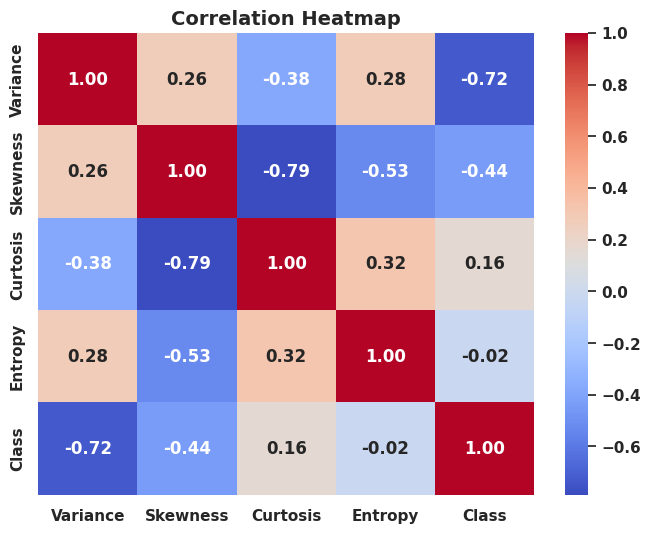
\includegraphics[width=0.7\textwidth]{Correlation.png}
\end{center}

Variance shows the strongest correlation with the target Class ($-0.72$), followed by Skewness ($-0.44$), indicating that these two features are the most discriminative for authenticity classification. Skewness and Curtosis are also strongly negatively correlated with each other ($-0.79$), suggesting some redundancy between the two.

\vspace{4mm}

\begin{center}
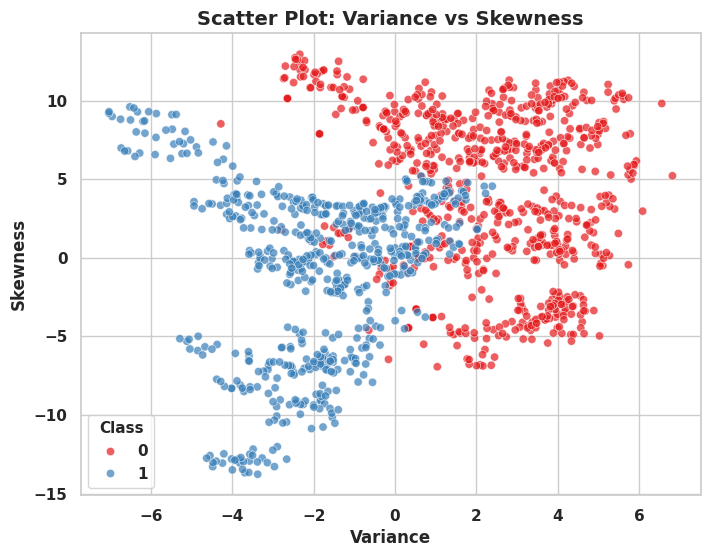
\includegraphics[width=0.65\textwidth]{Scatter.png}
\end{center}

The scatter plot of Variance versus Skewness shows that the two classes occupy largely distinct regions of the feature space, with authentic notes (Class 0) trending toward higher Variance and Skewness and forged notes (Class 1) clustering toward lower or negative values. There remains a region of overlap near the centre of the plot, which explains the small number of misclassifications observed during evaluation.

\vspace{4mm}

\begin{center}
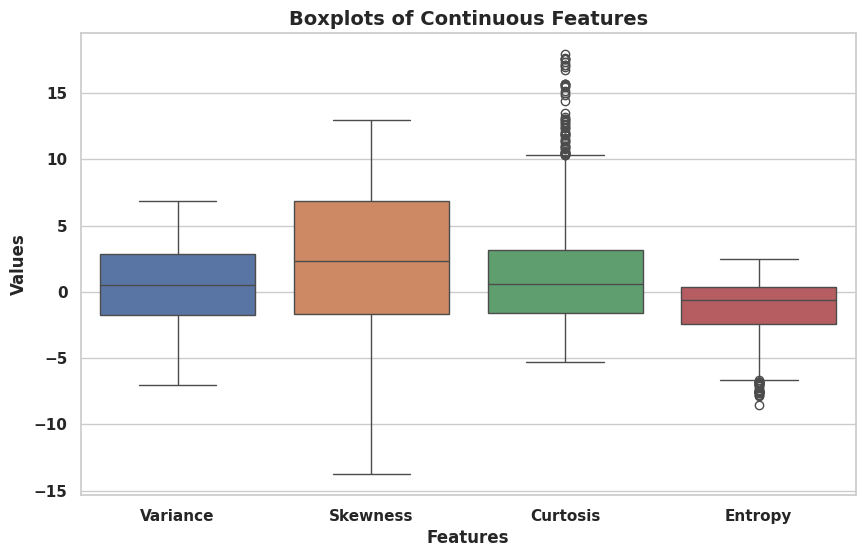
\includegraphics[width=0.75\textwidth]{Boxplots.png}
\end{center}

The boxplots show that Curtosis contains a considerable number of outliers with large positive values, while Entropy has a smaller cluster of low-value outliers; Variance and Skewness show no extreme outliers. Skewness also exhibits the widest interquartile range of the four features, consistent with the broad, right-skewed distribution seen in its histogram.

\vspace{4mm}

\begin{center}
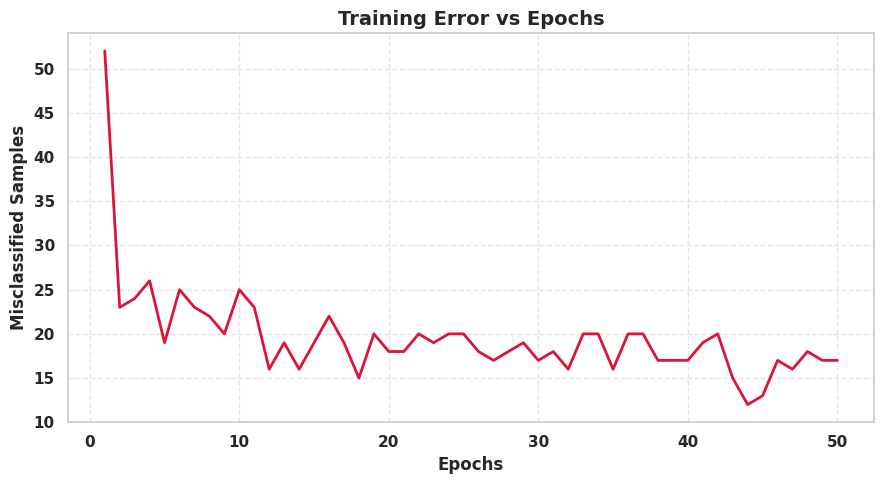
\includegraphics[width=0.75\textwidth]{error_vs_epochs.png}
\end{center}

Training error drops steeply from 52 to roughly 20 misclassified samples within the first two epochs and then oscillates in a narrow band between about 12 and 25 for the remaining epochs. This indicates that the dataset is not perfectly linearly separable, so the perceptron does not converge to zero error but instead stabilizes around a low, near-constant error rate.

\vspace{4mm}

\begin{center}
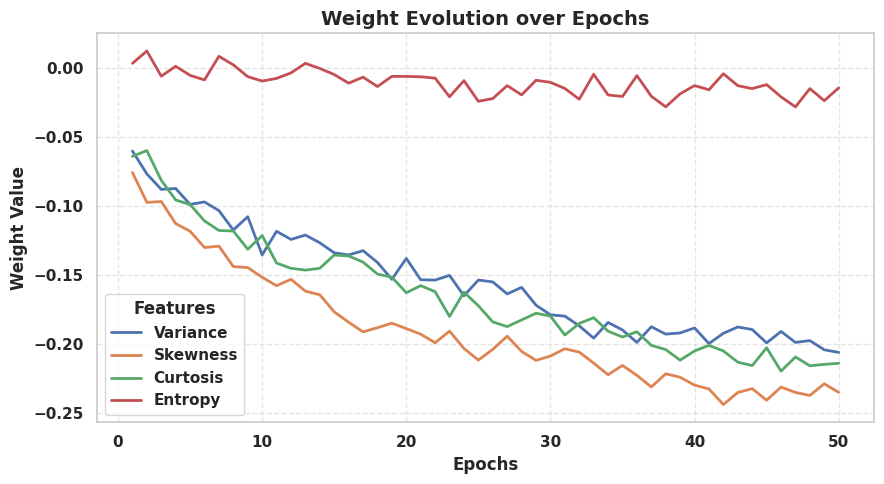
\includegraphics[width=0.75\textwidth]{weight_evolution.png}
\end{center}

The weights for Variance, Skewness and Curtosis steadily decrease and become increasingly negative over the 50 epochs, with the Skewness weight attaining the largest magnitude (approximately $-0.23$), reflecting its importance in the decision boundary. The Entropy weight remains close to zero throughout training, consistent with its near-zero correlation ($-0.02$) with the target class observed in the correlation heatmap.

\vspace{4mm}

\begin{center}
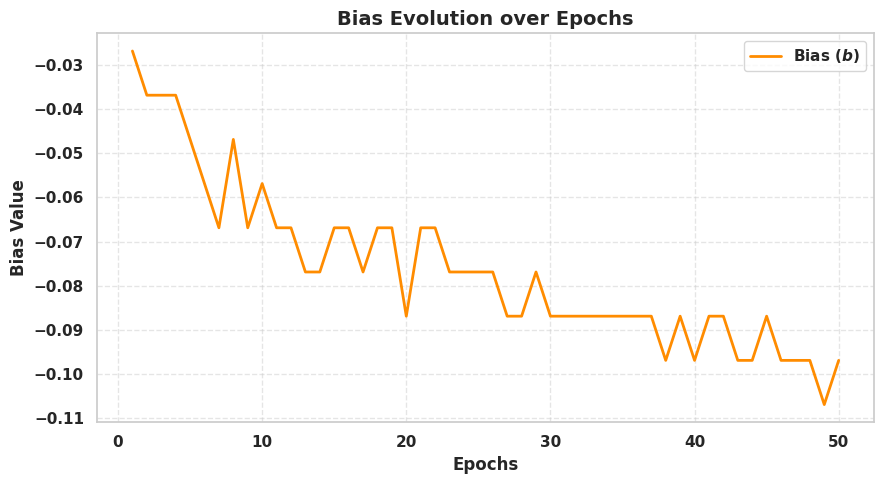
\includegraphics[width=0.75\textwidth]{bias_evolution.png}
\end{center}

The bias decreases steadily from about $-0.03$ to around $-0.10$ over the course of training, following the same oscillatory-but-decreasing trend seen in the weights. This shift in bias works together with the learned weights to move the decision boundary into a position that better separates the two classes.

\vspace{4mm}

\begin{center}
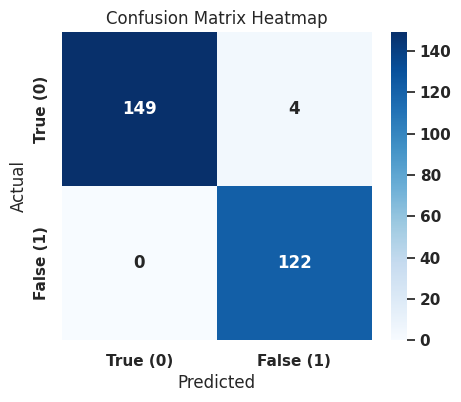
\includegraphics[width=0.55\textwidth]{Confuusion_matrix.png}
\end{center}

The confusion matrix shows 149 true negatives and 122 true positives, with only 4 false positives and zero false negatives on the test set. The absence of false negatives means the perceptron never failed to detect a forged note, though it occasionally misclassified a genuine note as forged.

\vspace{4mm}

\begin{center}
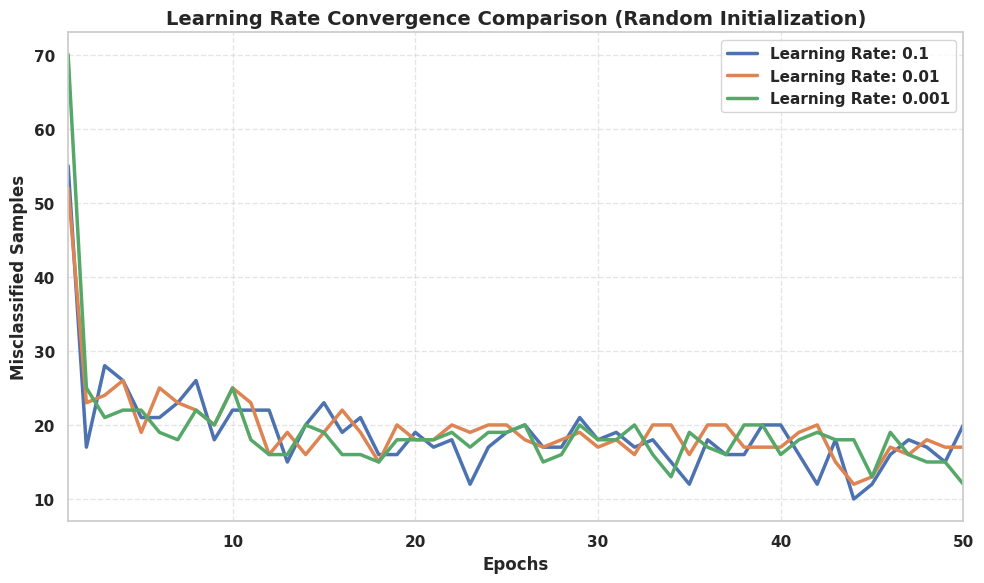
\includegraphics[width=0.75\textwidth]{learning_rate.png}
\end{center}

All three learning rates (0.1, 0.01 and 0.001) converge to a similar steady-state error band of roughly 15--20 misclassified samples after about 15--20 epochs, showing that the perceptron's final performance is not highly sensitive to the learning rate on this dataset. The larger learning rate (0.1) shows slightly more oscillation in the early epochs due to its larger update steps, while the smallest rate (0.001) produces a smoother and slightly slower initial descent.

%----------------------------------------------------------

\section*{7. Performance Tables}

\textbf{Training Summary}

\begin{tabular}{|p{6cm}|p{7cm}|}
\hline
Dataset Size & 1372 samples (5 columns)\\
\hline
Train/Test Split & Training: 1097 samples (80\%) \textbar\ Testing: 275 samples (20\%)\\
\hline
Learning Rate & 0.01\\
\hline
Epochs & 50\\
\hline
Final Weights & Variance: $-0.2058$, Skewness: $-0.2347$, Curtosis: $-0.2137$, Entropy: $-0.0144$\\
\hline
Final Bias & $-0.0969$\\
\hline
Accuracy & 98.5455\%\\
\hline
Precision & 96.8254\%\\
\hline
Recall & 100.0000\%\\
\hline
F1-score & 98.3871\%\\
\hline
\end{tabular}

\vspace{3mm}

\textbf{Epoch-wise Learning}

\emph{Weight 1 corresponds to Variance and Weight 2 corresponds to Skewness; the full four-feature weight vector at the final epoch is given in the Training Summary above.}

\begin{tabular}{|c|c|c|c|c|}
\hline
Epoch & Errors & Weight 1 & Weight 2 & Bias\\
\hline
1 & 52 & $-0.0601$ & $-0.0756$ & $-0.0269$\\
10 & 25 & $-0.1353$ & $-0.1515$ & $-0.0569$\\
20 & 18 & $-0.1378$ & $-0.1886$ & $-0.0869$\\
30 & 17 & $-0.1786$ & $-0.2085$ & $-0.0869$\\
40 & 17 & $-0.1881$ & $-0.2295$ & $-0.0969$\\
50 & 17 & $-0.2058$ & $-0.2347$ & $-0.0969$\\
\hline
\end{tabular}

%----------------------------------------------------------

\section*{8. Discussion and Conclusion}

The Single Layer Perceptron implemented from scratch was able to learn a near-linear decision boundary that separates authentic from forged banknotes with high accuracy. The correlation analysis and scatter plot confirmed that Variance and Skewness are the most discriminative features, and this was reflected in the trained model, where these two features received the largest-magnitude weights while Entropy remained close to zero throughout training. The training error curve showed rapid initial improvement followed by persistent oscillation rather than convergence to zero, indicating that the classes are only approximately, and not perfectly, linearly separable, which is consistent with the residual overlap visible in the scatter plot. The learning rate comparison further showed that the final performance of the perceptron is not highly sensitive to the choice of learning rate on this dataset, with all three rates settling into a similar error band.

On the held-out test set, the model achieved an accuracy of 98.55\%, a precision of 96.83\%, a recall of 100\%, and an F1-score of 98.39\%, with zero false negatives and only four false positives. This indicates that the perceptron is highly reliable at detecting forged notes, at a small cost of occasionally flagging genuine notes as forged. In conclusion, this experiment demonstrates that even a simple, single-layer, linear classifier can achieve strong performance on a well-structured, largely linearly separable dataset such as Banknote Authentication, while also illustrating the inherent limitations of the perceptron model when class boundaries are not perfectly linear.

%----------------------------------------------------------

\section*{9. References}

\begin{enumerate}
\item F. Rosenblatt, ``The Perceptron,'' \emph{Psychological Review}, 1958.
\item I. Goodfellow, Y. Bengio and A. Courville, \emph{Deep Learning}, MIT Press, 2016.
\item C. M. Bishop, \emph{Pattern Recognition and Machine Learning}, Springer, 2006.
\item S. Haykin, \emph{Neural Networks and Learning Machines}, Pearson, 2009.
\item UCI Machine Learning Repository -- Banknote Authentication Dataset.
\item Scikit-learn Documentation: Perceptron.
\end{enumerate}

\end{document}